\documentclass{article}
\title{人工智能导论作业1: Bait Game}
\author{王炳旭 221240001  email: 221240001@smail.nju.edu.cn}
\usepackage{ctex}
\usepackage{graphicx}
\usepackage{pifont}
\usepackage{geometry}
\usepackage{hyperref}
\hypersetup{hidelinks,
	colorlinks=true,
	allcolors=blue,
	pdfstartview=Fit,
	breaklinks=true}
\geometry{a4paper, left=2cm, right=2cm, top=3cm, bottom=3cm}
\begin{document}
\maketitle
{\fangsong (南京大学 \qquad  匡亚明学院 \qquad 南京\qquad 210093)}

{\heiti 摘\quad 要:} {\fangsong 使用深度优先搜索(DFS),深度受限搜索(LDS)以及$A^{*}$搜索实现对Bait Game的搜索. 并对Task4所涉及的蒙特卡洛树(MCTS)搜索进行分析解释.}

{\heiti 关键词:} {\fangsong 深度优先搜索, 深度受限搜索, $A^{*}$算法, 蒙特卡洛树搜索}

\section{深度优先搜索}
\begin{figure}[htbp]
\begin{minipage}[t]{0.5\linewidth}
\centering
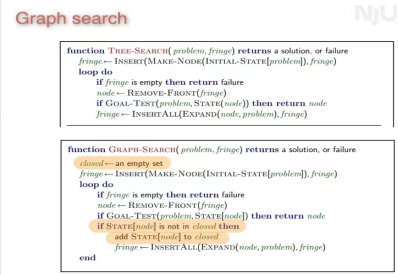
\includegraphics[width=0.9\textwidth]{DFS}
\centerline{(a) DFS}
\end{minipage}%
\begin{minipage}[t]{0.5\linewidth}
\centering
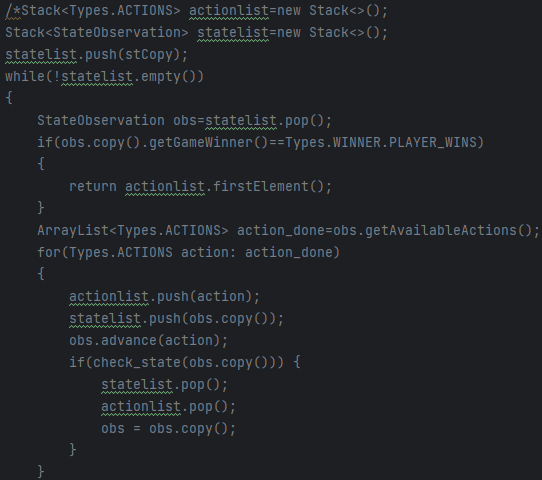
\includegraphics[width=0.9\textwidth]{Stack_DFS}
\centerline{(b) Stack-DFS}
\end{minipage}
\caption{DFS}
\end{figure}
深度优先算法的伪代码如图所示, 图中所示的方法是使用栈来实现DFS.但是在我实现的过程中, 出现了一些问题尚未解决.所以我又重新选择了递归作为实现DFS的媒介.原来使用栈的代码见图:

不论是递归还是使用栈来实现DFS, 原理都是一样的.下面使用代码分析递归的DFS:

\newpage
\begin{figure}
\centering
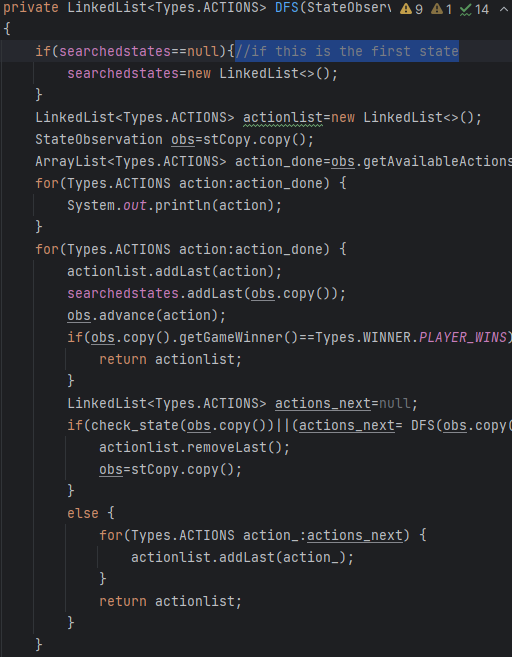
\includegraphics[width=0.6\linewidth]{DFS-recursion}
\caption{DFS-recursion}
\end{figure}

在递归DFS中, 我首先定义了用于储存搜索过程中的actions和states, 分别为searchedstates和searchedactions两个变量.接着在act函数中调用DFS函数进行深度优先搜索.由于不限制搜索深度, 所以每一次搜索将会进行至游戏胜利为止.

进入DFS函数后, 会使用actionlist变量对本次调用时所执行的动作行为操作进行储存.结束时, 返回这个actionlist.接着将当前游戏状态stCopy进行copy并加入到searchedstate变量中表示这是当前状态的下一个状态(中间的转换动作,即action由getAvailableActions()方法给出. 

接着,遍历当前状态可获得的所有动作,即$action_done$变量中的元素,并对obs.copy()使用advance()方法,让它"虚拟地"跑起来.运行完advance方法后, 需要判断执行后的状态是否是目标状态.如果是, 则说明我们已经找到从当前状态到达终点的路径.这时只需要返回actionlist就可以了. 如果当前状态不是终点状态, 那么就需要继续递归下去.但是,前提是当前状态不是我们已经搜索过的状态同时,该状态可以继续向下搜索.也就是代码中第三个if语句的内容.这时说明当前状态invalid, 需要剔除,同时恢复为原来的状态(对应"obs=stCopy.copy()"语句.

如果当前状态是个新的状态同时可继续向下搜索,则将搜索到的动作存储到$actions_next$变量中,并将其逐个添加到actionlist中.最后返回actionlist作为搜索结果.并在act函数中返回我们搜到的路径的第一个动作.

\section{深度受限搜索}
深度受限搜索在Task1的基础上对递归的深度进行了限制.我设置的最大搜索深度为5.(因为从Task1的运行来看, 关卡1所需要的搜索层数为10,所以设置对半深度,这样的话,正好使得avatar获得钥匙时达到最大搜索深度.)

相比于DFS, 我在深度受限搜索中多添加了heuristic-min-distance, bestactions, keyPosition, goalPosition等变量.
\begin{figure}[h]
\centering
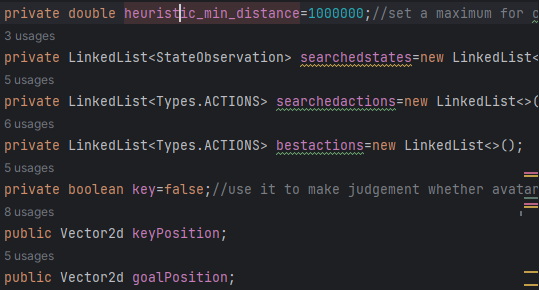
\includegraphics[width=0.6\linewidth]{LDS-variables}
\caption{LDS variables}
\end{figure}

这些变量的作用分别是:

\ding{172} heuristic-min-distance 用于表示当前搜索状态下的未来cost, 每一次搜索都会使用heuristic-distance函数对从当前状态走到终点状态所需花费的distance进行计算,如果比已有的距离还要小,那么这个方案比原有的搜索结果更好,这时就需要将当前的搜索路径searchedactions克隆给bestactions变量.

\ding{173} bestactions变量是用于记录从当前真实状态到达已搜索的最后状态之间的最佳路径.因为从当前状态到达搜索出的最终状态可能有多种路径, 这时候就需要我们找开销最小的路径进行执行.也就是前面所说的heuristic-min-distance变量的作用.

\ding{174} 由于avatar需要先得到钥匙然后再到达大门gate处.所以在计算未来cost时要考虑avatar是否已经拿到钥匙.这需要设置key变量来表示当下avatar是否已经拿到钥匙.(好像框架函数本身具有判断avatar是否拿到钥匙的内容.)

\ding{175} keyPosition和goalPosition分别是钥匙和大门的位置, 获取方式与作业要求中的方式相同.

接下来是对代码的分析:

LDS与DFS最大的不同点在于限制了最大搜索深度.当搜索到达最大深度且未至终点时,需要将已搜索到的最优方法返回到bestaction中.这需要在原来DFS的代码基础上, 多引入current-depth变量来记录当前搜索的深度,这个参数随着搜索的深入而不断减小. 当减小到0时,就需要计算到达终点状态还需要多少cost, 最终选择出最佳路径并执行.其余部分与DFS所差无几.
请看详细代码:
\begin{figure}[htbp]
\begin{minipage}[t]{0.5\linewidth}
\centering
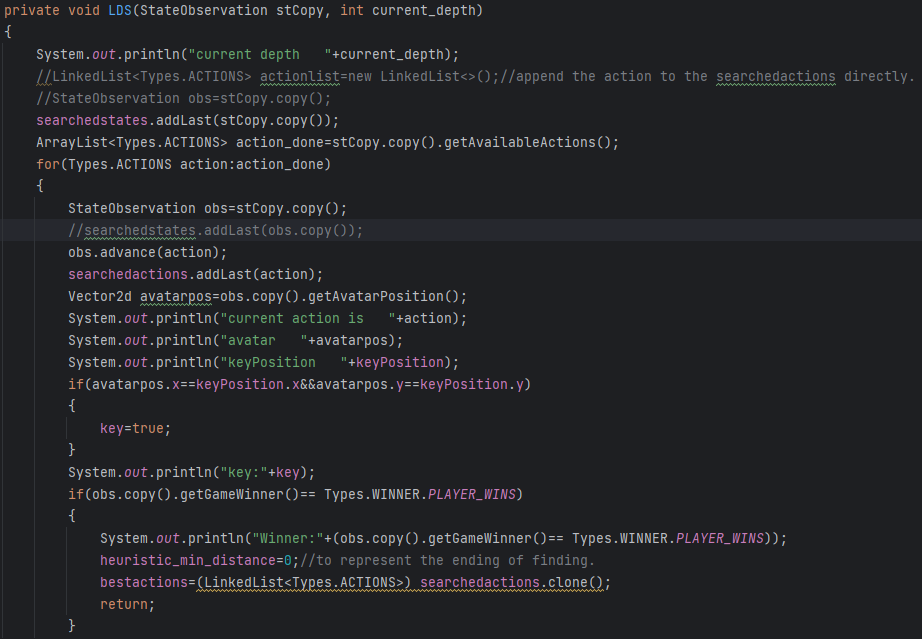
\includegraphics[width=0.9\textwidth]{LDS1}
\centerline{(a) LDS1}
\end{minipage}%
\begin{minipage}[t]{0.5\linewidth}
\centering
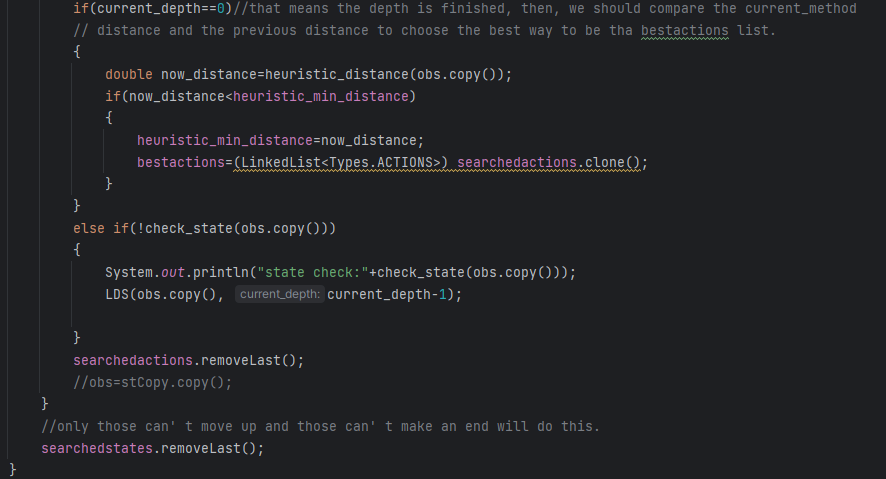
\includegraphics[width=0.9\textwidth]{LDS2}
\centerline{(b) LDS2}
\end{minipage}
\caption{LDS}
\end{figure}

对于其中计算heuristic-min-distance的过程, 使用函数"heuristic distance"函数进行计算, 这里计算两个网格的曼哈顿距离.
\begin{figure}
\centering
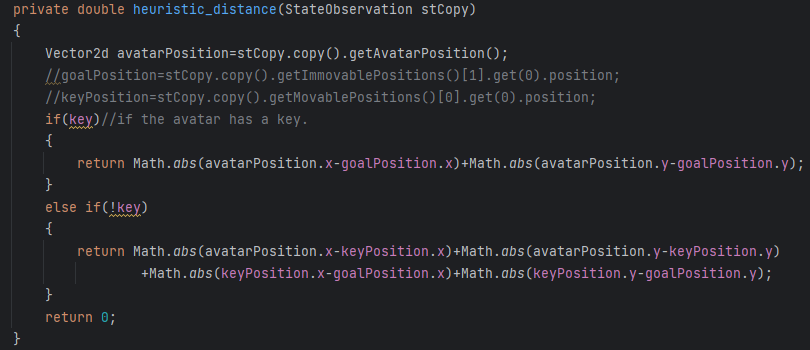
\includegraphics[width=0.6\linewidth]{heuristic LDS}
\caption{Heuristic distance}
\end{figure}

\newpage
\section{$A^{*}$算法}
$A^{*}$算法是启发式搜索算法,考虑了当前状态的过去cost与未来cost作为决策依据.其核心是表达式:$$F=G+H$$
其中, H是启发式函数.在本任务中, H函数是当前状态到终点状态的cost加上已有的场上分数以及箱子和洞配对的分数构成.为什么设置这样的启发函数, 因为avatar必须推箱子到洞中,才有可能有路径到达key或大门.这时候就必须考虑箱子和洞口的配对.由于并不知道avatar会推动哪一只箱子,所以在计算的时候,将所有的箱子和洞口进行计算.相关过程在heuristic-distance和box-and-hole函数中实现.

其次, 实现$A^{*}$需要使用优先级队列PriorityQueue.所以我参考了网络上对于Java中PriorityQueue的使用.(\href{https://blog.csdn.net/qq\_45978890/article/details/115802114?ops\_request\_misc=\%257B\%2522request\%255Fid\%2522\%253A\%2522169608481316800184148350\%2522\%252C\%2522scm\%2522\%253A\%252220140713.130102334..\%2522\%257D\&request\_id=169608481316800184148350\&biz\_id=0\&utm_medium=distribute.pc_search_result.none-task-blog-2~all~sobaiduend~default-1-115802114-null-null.142^v94^insert\_down28v1\&utm_term=Java\%20Astar\&spm=1018.2226.3001.4187}{参考资料})
详细PriorityQueue的实现间下方代码:

\ding{172} 首先是节点Node的实现, 根据我查阅的参考资料, 需要从JAVA本身自带的Node类复写继承来实现对每一个搜索状态中所需要的各种数据进行存储. 这个Node是implement自Node类.里面所需要的各种成员数据如下:
\begin{figure}[h]
\centering
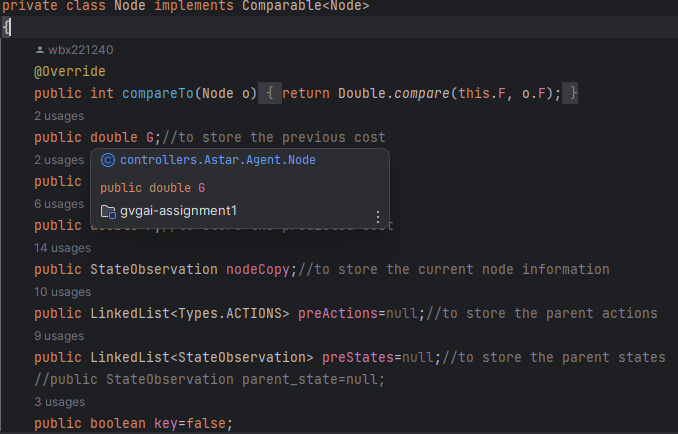
\includegraphics[width=0.5\linewidth]{Node}
\caption{Node implement}
\end{figure}

图中给出了Node类中所包含的一些成员对象: nodeCopy表示当前节点的全局状态; preActions用于表示到当前状态所需要的动作,类型是LinkedList<Types.ACTIONS>; preStates是当前节点的父亲节点们; key用于表示当前节点状态是否拿到了钥匙.在下面的图中还有一个AvatarPosition变量用于表示当前节点下avatar的位置.
\begin{figure}[h]
\centering
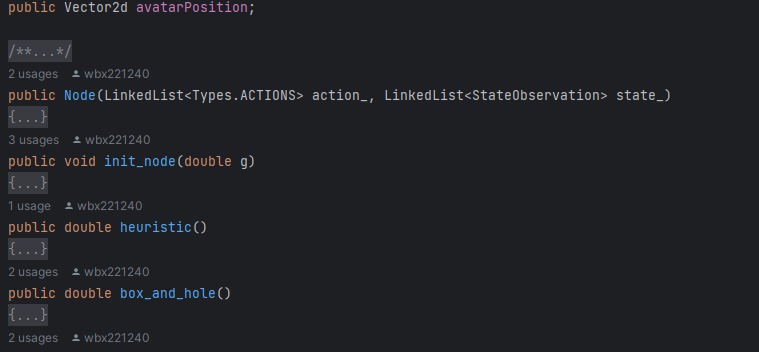
\includegraphics[width=0.5\linewidth]{Node1}
\caption{Node implement1}
\end{figure}

\newpage

在上图中, 每当我们需要 新建一个节点时都需要调用"new Node()", 传入的参数是当前节点的preActions和preStates.同时还需要调用"init-node()"函数进行启发值F,G, H的计算, 传入参数为G,即前序开销.

"heuristic()"函数是计算启发式函数H的函数.它的计算方法是用曼哈顿距离计算avatar走到Win状态所需的开销加上过程中推箱子进洞的开销以及当前状态的场上得分. "box-and-hole"函数就是计算推箱子开销的.

\ding{173}一些全局性的变量:
\begin{figure}[h]
\centering
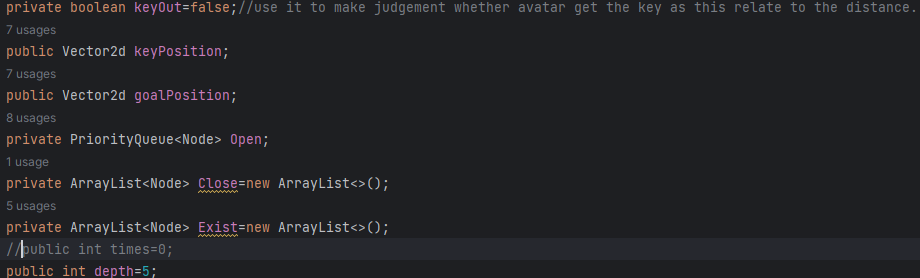
\includegraphics[width=0.5\linewidth]{Node2}
\caption{Variables}
\end{figure}
两个位置变两个用于表示门和钥匙的位置,;Open为优先级队列,是搜索的核心, 所有的搜索节点都会加入到Open中, 每次循环poll出其中优先级最高的一个节点用于作为当前节点进行下一步搜索;Close列表用于存储被搜索过的节点;Exist列表用于存储所有节点,包括在Open列表中的节点.

\ding{174} 有关act函数的相关内容:

\begin{figure}[h]
\centering
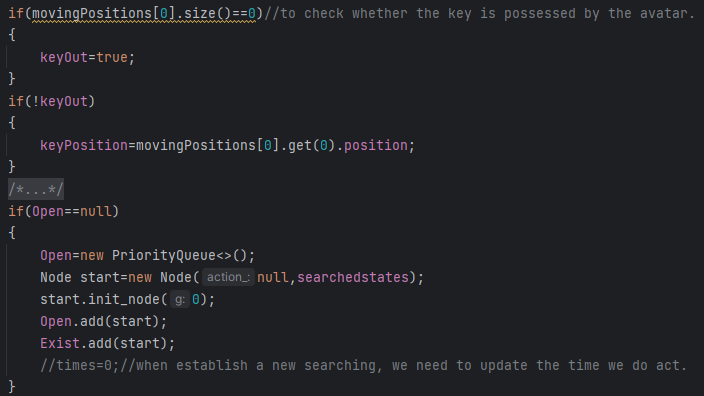
\includegraphics[width=0.5\linewidth]{Astaract}
\caption{Act}
\end{figure}

在图中可以看到, 如果钥匙已经被拿走, 那么就不许要再获取钥匙的位置了. 这时设置keyPosition为TRUE. 

图中第三个if语句较为关键,当我们第一次进行搜索的时候,Open队列中是没有东西的(因为在定义Open队列时做了区分, 初值为null). 此时就需要根据当前的stCopy进行构建第一个Node, 并加入到Open里面.

\begin{figure}[h]
\centering
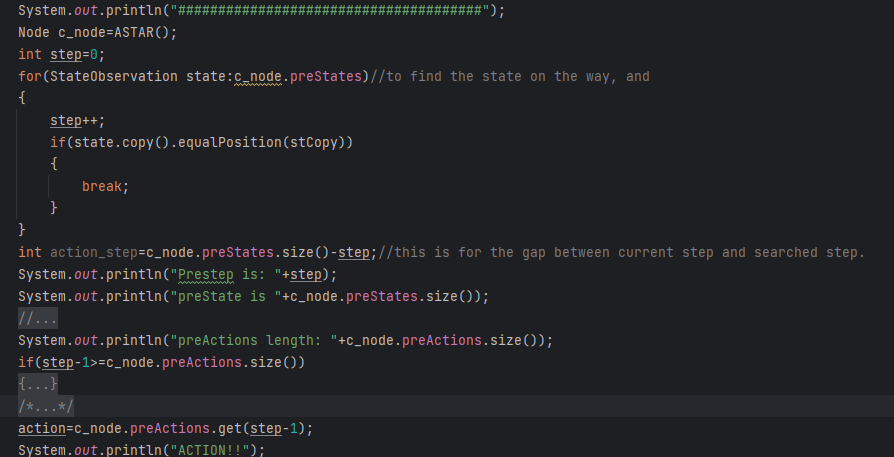
\includegraphics[width=0.5\linewidth]{act1}
\caption{act1}
\end{figure}

在这里, 我的想法是用ASTAR这个函数来返回搜索到的最后一个节点. 因为Node中包含着搜索的全部信息, 比单独返回actionlist和statelist要跟有用. 当然, 我前几次尝试的时候用的仍然是返回动作列表的形式.但是我发现一个问题, 就是无法精确定位到当前状态应该act哪一个动作. 仅仅返回了一系列动作而没有返回确切应该执行哪一个动作. 所以我使用Node作为返回值. 然后计算从当前状态stCopy到达搜索的中止状态需要的步骤数, 根据步骤数得到准确的action.这就是我在代码中实现的部分. 使用一个\textit{for}循环得到父亲状态中和它一样的状态的位置(step)然后,根据这个step去preAction中找到下一步的action. 这就是代码中$$"action=c-node.preActions.get(step-1)"$$ 这一句所做到的事情.

\textbf{但是, 我还发现一个问题:}\textit{preActions的长度往往不会大于preStates的长度, 也就是说父亲节点中多出来一些无关的节点, 我的想法是可能是在Astar算法运行过程中出现的问题.} 为了不影响正常搜索, 我在里面多加了一个判断, 防止下标出界.

\ding{175} Astar的主体:

\begin{figure}[h]
\centering
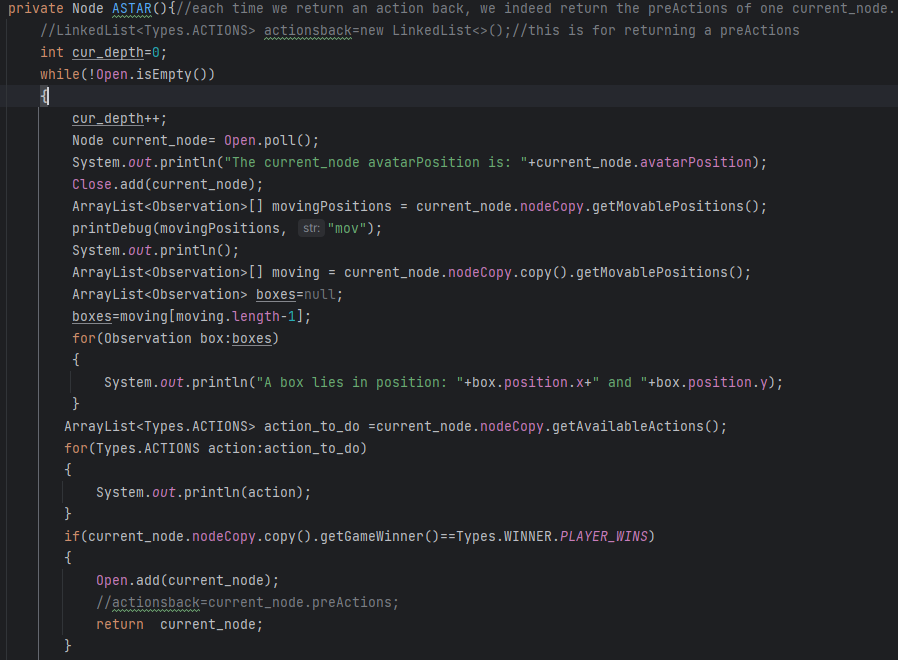
\includegraphics[width=0.5\linewidth]{Astar}
\caption{astar}
\end{figure}

在ASTAR中我先设置了当前搜索的深度cur-depth, 其值不会超过5,当深度受限时, 便会自动停止并返回当前的节点current-node.
然后按照ASTAR的正常流程进行搜索. 里面需要注意的是,由于Open列表的元素都是Node, 对于我们不需要的或不符合要求的节点我们不想把它加到Open队列里面.所以这时候先对当前的状态obs-next再进行一次copy.\textit{这一操作的目的是为了更进一步地判断当前状态advance后是否符合要求.} 

本来是没有这一操作的, 但是我发现在试运行的时候,avatar就会按照已经搜过的路径进行行动,返回一步步检查的时候发现的问题.

其余不用多讲.
\begin{figure}
\centering
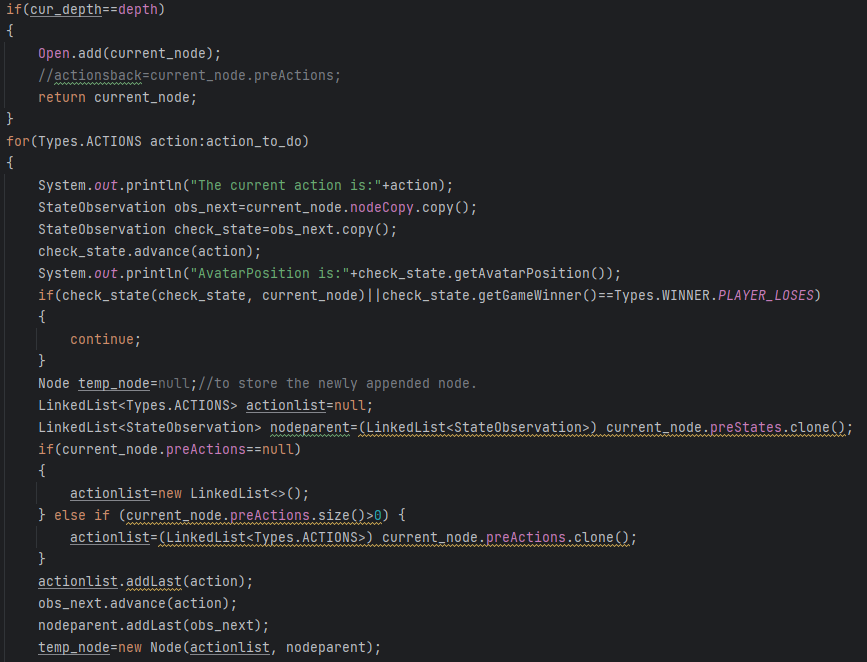
\includegraphics[width=0.5\linewidth]{ASTAR2}
\caption{ASTAR2}
\end{figure}

\begin{figure}
\centering
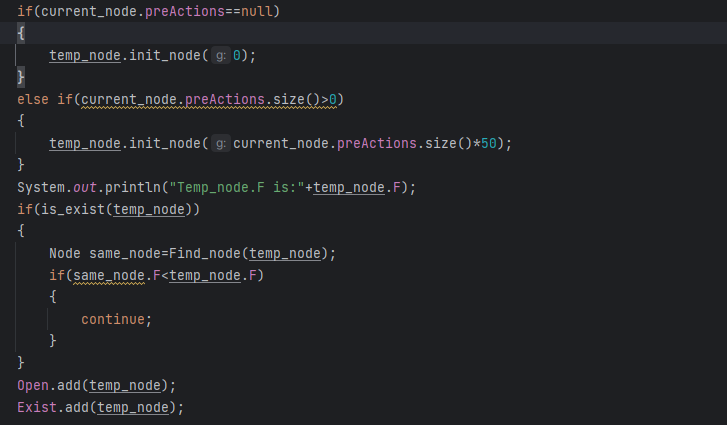
\includegraphics[width=0.6\linewidth]{ASTAR3}
\caption{ASTAR3}
\end{figure}
在新建Node的时候需要考虑当前Node是否已经被搜索过, 如果是的, 那么就比较两次不同搜索时的H值的大小进行选择最优的搜索方式.
\section{蒙特卡洛树搜索}
蒙特卡洛树搜索属于强化学习中的随机性算法.通过阅读代码, 可知: 其搜索思路是先在给定的搜索深度下进行搜索, 然后使用rollOut函数来获得关于已搜索的结点的信息并进行回溯.

\ding{172}在"SimpleMCTS/Agent.java"文件中, 依然由act函数返回经过MCTS后获得的可执行动作action.但是不同的是, 这个action由run函数得到. 在"SingleMCTSPlayer.java"文件中, run函数的功能是在给定的时间内完成MCTS并返回action.时间由参数elapsedTimer给出.

但是, run函数中还调用了mostVisitedAction或bestAction来对所获取的action进行选择, 得到最优动作.

\ding{173}执行MCTS的主要过程是"SingleTreeNode.java"中的mctsSearch方法.这个方法中包含一个主循环while用于控制搜索的时间和深度.在循环中, 不断使用treePolicy()方法展开当前节点的下一步可执行动作以及对应的结点.但是, 它做的并不只是随机展开当前节点. 如果当前节点未被展开过, 那么只需要展开就好了. 但是, 如果此节点先前已经展开过了, 那么就需要通过一定的比较方法,得到最优展开方式.这种判断方法就是UTC或者是Epsilon-Greedy().  (UTC是计算当前节点的UTCvalue与设置的bestvalue进行比较,需要注意的是代码中还使用Utils.noise对数据进行噪声处理,防止出现相同的UTCvalue)

\ding{174}接着使用rollOut函数随机获取value以及action.

\ding{175}最后使用backup函数记录从rollOut函数中得到的value并不断回溯以改变前序节点的value.然后进行下一次的结点选择直至深度受限或时间受限.
\end{document}
